\documentclass[12pt]{elsarticle}
%\usepackage[centertags]{amsmath}
\usepackage{amsmath}
\usepackage{amsfonts}
\usepackage{amssymb}
\usepackage{amsthm}
\usepackage{color}
\usepackage{graphicx}
%\usepackage{subfigure}
\usepackage{epsfig,mathrsfs}
\usepackage[bf,SL,BF]{subfigure}
\usepackage{fancyhdr}

%\usepackage{CJK}
\usepackage{caption}
\usepackage{wrapfig}
\usepackage{cases}
\usepackage{algorithm}
%\usepackage{algorithmic}
\usepackage{algpseudocode}
\usepackage{multirow}
% THEOREM Environments --------------------------------------------------------
\newtheorem{thm}{Theorem}[section]
\newtheorem{cor}[thm]{Corollary}
\newtheorem{lem}[thm]{Lemma}
\newtheorem{prop}[thm]{Proposition}
\theoremstyle{definition}
\newtheorem{defn}[thm]{Definition}
\theoremstyle{remark}
\newtheorem{rem}[thm]{Remark}
\numberwithin{equation}{section}
% New command ----------------------------------------------------------------
\newcommand{\fai}{\pmb{\phi}}
\newcommand{\pai}{\pmb{\pi}}
\newcommand{\q}{\textbf{\emph{q}}}
\newcommand{\p}{\textbf{\emph{p}}}
\newcommand{\x}{\textbf{\emph{x}}}
\newcommand{\bm}[1]{\emph{\textbf{#1}}}
\newcommand{\n}{\textbf{n}}
\newcommand{\R}{\mathcal{R}}
\newcommand{\RL}{Riemann-Liouville }
\newcommand{\cinf}[1]{C_0^{\infty}(#1)}
\newcommand{\abs}[1]{\left\vert#1\right\vert}
\newcommand{\set}[1]{\left\{#1\right\}}
\newcommand{\seq}[1]{\left<#1\right>}
\newcommand{\norm}[1]{\left\Vert#1\right\Vert}
\newcommand{\flux}[1]{\widehat{{#1}}}
%\newcommand{\essnorm}[1]{\norm{#1}_{ess}}
\makeatletter
\newcommand{\rmnum}[1]{\mathcal{\romannumeral #1}}
\newcommand{\Rmnum}[1]{\mathcal{\expandafter\@slowromancap\romannumeral #1@}}
\makeatother

\begin{document}

\pagenumbering{arabic}

\begin{frontmatter}
\title{{\bf  Local nodal discontinuous Galerkin methods for fractional equations on 2D domain with triangular meshes}}
\author{Liangliang Qiu, Weihua Deng$^{1,*}$, Jan S. Hesthaven}
\cortext[cor2]{Corresponding author. E-mail: dengwh@lzu.edu.cn.}
\address{$^1$School of Mathematics and Statistics,
Lanzhou University, Lanzhou 730000, P. R. China}

%\date{}

\begin{abstract}
This paper, as the sequel to our previous work, develops numerical schemes for fractional diffusion equations on a two-dimensional finite domain with triangular meshes.  We adopt the local nodal discontinuous Galerkin methods for the full spatial discretization by the use of high-order nodal basis, employing multivariate Lagrange polynomials defined on the triangles. Stability analysis and error estimates are provided in the higher dimensional cases.
Finally, numerical experiments show the optional order of convergency.

\noindent {\bf Keywords:}
2D fractional diffusion equation; triangular meshes; local nodal discontinuous Galerkin methods.
\end{abstract}
\end{frontmatter}

\section{Introduction}
Historically fractional calculus came out nearly in the same time with classical calculus. As a natural extension of classic calculus, its application and development like fractional partial differential equations(FPDEs) are not so mature as that associated with classic calculus. It is until the last few decades that fractional calculus begun to apply to describe a wide range of non-classical phenomena such as applied science and engineering, for example the fractional Fokker-Planck equations for anomalous diffusion problems and continuous time random walk models(\cite{barkai}, \cite{metzler}), and  the subdiffusion and superdiffusion process.

With the increasing utilization of fractional calculus in a series of models, it is necessary to propose appropriate and robust numerical methods for solve FPDEs for practical application. A fundamental difference between problems in classic calculus and fractional calculus lies in the fact that factional operators are non-local and have a character of history independence, causing the essential difficulties and challenges for numerical approximation.

In recent years, however, there came out a few successful work to deal with discretizing fractional models by applying traditional numerical schemes, including finite difference method, finite element method, and spectral method. Meerschaert and Tadjeran in [12] firstly proposed a stable difference method-the shifted Gr\"{u}nwald-Letnikov formula to approximate fractional advection-dispersion flow equations. And recently, Tian et al.  put forward a higher accurate numerical solution
of the space fractional diffusion equation, named the weighted and shifted Gr��nwald difference operators. In \cite{xu1}, Xu and his coworker considered a space-time spectral method for solving the time fractional diffusion equation. Deng\cite{deng1} developed the finite element method for discretizing the space and time fractional Fokker-Planck equation.

Another high order accurate numerical method-discontinuous Galerkin method also began to attract a great attention, and several attempts had been tried very recently. In 2010, Deng and Jan \cite{deng2} proposed a local discontinuous Galerkin method for the fractional diffusion equation, and also gave stability analysis and error estimates, confirming that the schemes could show optional order of convergence for the superdiffusion case. Almost in the same time, Ji and Tang\cite{xia} presented  a purely qualitative study of the solution of spatial Caputo fractional problems in one and two dimensions using a high-order Runge-kutta discontinuous
Galerkin methods, but failed to offer theoretical results.

The main advantages of DG methods include: ensuring geometric flexibility and supporting for locally adapted resolution as well as excellent parallel efficiency. In \cite{xia}, the authors adopted the rectangular meshes to deal with the two-dimensional cases, which lost one of the most important benefits of DG methods. This paper, as a subsequence of out previous work \cite{deng2}, will discuss how to approximate fractional diffusion equations with unstructured grids beyond one dimension in detail and give theoretical analysis in higher dimensional frame. In order to focus on how to overcome the difficulties of developing LDG for fractional problems with unstructured meshes, we only consider left \RL fractional equations.


The paper is organized as follows. In section 2, we review the definitions of fractional operators and fractional functional setting. In the next section, we propose our numerical schemes and show the detailed algorithm in computation. Section 4 gives the corresponding stability analysis and error estimates. Some conclusions are given in the last section.

\section{Preliminaries}
In this section, we make some preparation including the definitions of fractional derivatives and associated functional setting for
the subsequent numerical schemes and theoretical analysis.
\subsection{Fractional calculus, norms and integral spaces}
First we recall some definitions of the left fractional derivatives and integrals listed as follows:
\begin{itemize}
  \item left \RL fractional derivative:
    $$ _aD_x^{\alpha}u(x) = \frac{1}{\Gamma(n-\alpha)} \frac{d^n}{dx^n} \int_{a}^{x} (x- \xi)^{n - \alpha -1}u(\xi) d\xi$$
  %\item right \RL fractional derivative:
%    $$ _xD_b^{\alpha}u(x) = \frac{(-1)^{n}}{\Gamma(n-\alpha)} \frac{d^n}{dx^n} \int_{x}^{b} (\xi - n)^{n - \alpha -1}u(\xi) d\xi$$
  \item left Caputo fractional derivative:
    $$ _a^{C}D_x^{\alpha}u(x) = \frac{1}{\Gamma(n-\alpha)}  \int_{a}^{x} (x- \xi)^{n - \alpha -1}{u^{(n)}(\xi)} d\xi$$
  %\item right Caputo fractional derivative:
%    $$ _{x}^{C}D_b^{\alpha}u(x) = \frac{(-1)^n}{\Gamma(n-\alpha)}  \int_{a}^{x} (\xi - x)^{n - \alpha -1}{u^{(n)}(\xi)} d\xi$$
  \item left fractional integral:
    $$ _aD_x^{-\alpha}u(x) = \frac{1}{\Gamma(\alpha)}  \int_{a}^{x} {(x-\xi)^{\alpha-1}}{u(\xi)} d\xi$$
%  \item right fractional integral:
%    $$ _xD_b^{-\alpha}u(x) = \frac{1}{\Gamma(\alpha)}  \int_{x}^{b} {(\xi-x)^{\alpha-1}}{u(\xi)} d\xi$$
\end{itemize}
where $\Gamma(\cdot)$ denotes Gamma function, $\alpha \in [n-1,n)$, $x\in(a,b)$, a and b can be $-\infty$ and $+\infty$ respectively.


According to the definitions of \RL fractional derivative and Caputo derivative, an importance equivalence can be obtained
\begin{equation}
_aD_x^{\alpha} u(x) =  {_a^C}D_x^{\alpha} u(x) \quad if \quad u^{k}(a) = 0, \quad k=0,1, \cdots, n-1,
\end{equation}
where n is the smallest integer greater than or equal to $\alpha$ and $u(x)$ is sufficiently smooth.
By simple linear transformations, fractional integral have an equivalent form, i.e.,
\begin{equation}
%\begin{split}
_aD_x^{-\alpha} u(x) = \frac{1}{\Gamma(\alpha)} ( \frac{x-a}{2} )^{\alpha} \int_{-1}^{1} (1-\eta)^{\alpha-1}u(\frac{x+a}{2} + \frac{x-a}{2}\eta) d\eta.
%_xD_b^{-\alpha} u(x) = \frac{1}{\Gamma(\alpha)} ( \frac{b-x}{2} )^{\alpha} \int_{-1}^{1} (1+\eta)^{\alpha-1}u(\frac{b+x}{2} + \frac{b-x}{2}\eta) d\eta.
%\end{split}
\label{eq2:2}
\end{equation}
On the basis of (\ref{eq2:2}), we use the Gauss-Jacobi quadrature with weight functions $(1-\eta)^{\alpha-1}$ to solve the weakly singular fractional integrals in numerical computation.
\begin{lem}
The left and right fractional integral operators are adjoint in the sense of the $L^2(a,b)$ inner product, i.e.,
\begin{equation}
(_aD_x^{-\alpha}u,v)_{L^2(a,b)} = (u,_{x}D_b^{-\alpha}v)_{L^2(a,b)}  \quad \forall \alpha>0, a<b
\end{equation}
\end{lem}
In order to carry out the analysis, we need to introduce the fractional integral spaces here.
\begin{defn}
Let $\alpha >0$. Define the norm
\begin{equation}
    \norm{u}_{H^{-\alpha}(\R)} :=  \norm{ |\omega|^{-\alpha} \widehat{u}}_{L^2(\R)}
\end{equation}
where $\widehat{u}(\omega)$ is the Fourier transform of $u(x)$ and let $H^{-\alpha}(\R)$ denote the closure of $\cinf{\R}$ with respect to $\norm{\cdot}_{H^{-\alpha}(\R)}$.
\end{defn}
\begin{defn}
Let  $\alpha>0$. Define the norm
\begin{equation}
\norm{u}_{J_{L}^{-\alpha}(\R)} := \norm{_{-\infty}D_x^{-\alpha}u}_{L^2{(\R)}}
\end{equation}
and let $J_{L}^{-\alpha}(\R)$ denote the closure of $\cinf{{\R}}$ with respect to $\norm{\cdot}_{J_L^{-\alpha}(\\R)}$.
%as well as the norm associated with the left fractional integral.
\end{defn}
\begin{defn}
Let $\alpha>0$. Define the norm
\begin{equation}
    \norm{u}_{J_R^{-\alpha}(\R)}  := \norm{_xD_{\infty}^{-\alpha}u}_{L^2(\R)}
\end{equation}
and let $J_R^{-\alpha}(\R)$ denote the closure of $\cinf{\R}$ with respect to $\norm{\cdot}_{J_L^{-\alpha}(\R)}$.
\end{defn}

\noindent The three norms are closely related as stated in the following result.
\begin{thm}
The three spaces $H^{-\alpha}$, $J_L^{-\alpha}$, and $J_R^{-\alpha}$ are equal with equivalent norms.
\end{thm}

Detailed proof can be found in \cite{deng2} and we omit it here.
\begin{lem}
\begin{equation}
    (_{-\infty}D_x^{-\alpha}u,\smallskip _xD_{\infty}^{-\alpha} u) = cos(\alpha \pi)\norm{D^{-\alpha}u}^2_{L^2(\R)} = cos(\alpha \pi) \norm{u}^2_{H^{-\alpha}(\R)}.
\end{equation}
\end{lem}
\noindent Let us now restrict attention to the case in which $ supp(v) \subset \Omega = (a,b)$. Then $_{-\infty}D_x^{-\alpha }u = {_a}D_x^{-\alpha}$,
and $_{x}D_{\infty}^{-\alpha} = {_x}D_b^{-\alpha}$. Straightforward extension of the definitions given above yields.
\begin{defn}
Define the spaces $H_0^{-\alpha}(\Omega)$, $J_{L,0}^{-\alpha}(\Omega)$, and $J_{R,0}^{-\alpha}(\Omega)$ as the closures of $\cinf{\Omega}$.
\end{defn}

The following theorem gives the relations among the fractional integral spaces with different $\alpha$ .
\begin{thm}
If $-\alpha_2 < -\alpha_1 < 0$, then $J_{L,0}^{-\alpha_1}(\Omega)$ $(H_0^{-\alpha_1}(\Omega)$ or $J_{R,0}^{-\alpha_1}(\Omega))$ is embedded into
$J_{L,0}^{-\alpha_2}(\Omega)$ $(H_0^{-\alpha_2}(\Omega)$ or $J_{R,0}^{-\alpha_2}(\Omega))$, and $L^2(\Omega)$ is embedded into both of them.
\end{thm}

\subsection{Notations for DG methods}
We consider problems posed on the physical domain $\Omega$ with boundary $\partial\Omega$ and assume that this domain is well approximated by
the computational domain $\Omega_h$.  Generally, we denote $\Omega_h$  with $\Omega$ if no misunderstanding is caused. This is a space filling triangulation composed of a collection of K geometry-conforming nonoverlapping elements, $D^k$, i.e.,
$$\Omega \simeq \Omega_h = \bigcup_{k=1}^{K}D^k,$$
and $\Gamma$ denotes the union of the boundaries of the elements $D^k$ of $\Omega_h$.
$\Gamma$ consists of two parts: the set of unique purely internal edges $\Gamma_i$ and the set of external edges $\Gamma_b=\partial \Omega$ of domain boundaries, and
$\Gamma = \Gamma_i\bigcup\Gamma_b$
The shape of these elements can be arbitrary although we will mostly consider cases where they are d-dimensional  curvilinear simplices. In the two-dimensional case, the planar triangles are adopted.

For the general curvilinear 2-simplex $D$, there exists a diffeomorphism $\Psi:D\rightarrow I$ where $I \in \R^2$ is the standard triangle with the three vertices, $(-1,-1)$, $(1,-1)$ and $(-1,1)$. In order to form the nodal basis on triangle, we just need to focus attention on the problem of interpolation in the triangle, $I$.

We now define the space of N-th-order polynomials in two variables, $P_N^2(D)$ such that the dimension of the approximation polynomial space is
$$ dim P_N^2(D) = N_p = \binom{N+2}{N}
$$
which is the minimum number that allow $P_N^2(D)$ to be complete. Here $N_p$ is the number of nodal set $\{\pmb{\xi}_i\}_{i=1}^{N_p}$ in $I$ or interchangeably $\{\pmb{x}_i\}_{i=1}^{N_p}$ in $D$. There are exactly $N+1$ nodal points along each of the three edges and they are also the members of the nodal set. Examples of such nodal points are provided in \cite{chen1} and \cite{jan2}.

The polynomial space $P_N^2(D)$ can be illustrated as
\begin{eqnarray}
P_N^2(D^k) &=& span\{x^iy^j \ |\ (i,j)\geqslant0, i+j \leqslant N, (x,y) \in D^k \} \nonumber \\
           &=& span\{ \ell_i^k(\x) \ | \  i= 1, 2,  \cdots, N_p, \ \x = (x,y) \in D^k \} \nonumber
\end{eqnarray}
where $\ell(\x)$ denotes the two-dimensional multivariate Lagrange interpolation basis function. For the details of the multivariate  higher-dimensional Lagrange
interpolation functions, we refer to \cite{jan1} and \cite{jan2}.

Let us finally define a number of different inner products on the curvilinear simplex, $D$. Consider the two continuous functions $f,g$, then the inner product, the associated $L_2$ norm and the inner product over the surface of D are defined as
$$
(f,g)_D = \int_D f(\x)g(\x) d\x, \quad (f,f) = ||f||_D^2, \quad (f,g)_{\partial D} = \int_{\partial D} f(\x) g(\x) d s .
$$
In the corresponding global broken measures, inner products and norms are
$$
(f,g)_{\Omega} = \sum_{k=1}^{K} (f,g)_{D^k}, \quad (f,f) = \sum_{k=1}^{K} ||f||_{D^k} = ||F||_{\Omega}, \quad (f,g)_{\Gamma} = \sum_{k=1}^{K} (f,g)_{\partial D^k}.
$$


%\begin{displaymath}
%\begin{split}
%
%\end{split}
%\end{displaymath}

%Let us finally define a number of different inner products on the curvilinear simplex, $D$. Consider the two functions,

Next, we introduce some notations to manipulate numerical fluxes. For $e\in \Gamma$, we refer to the interior information by a superscript "+" and to the exterior information by a superscript "-".
Using these notations, it is useful to define the average
$$\{u\} = \frac{u^++u^-}{2} \quad on \ e\in \Gamma_i,$$
$$ \{u\} = u \quad on \ e \in \Gamma_b $$
where $u$ can be both a scalar and a vector.
In a similar fashion, awe also define the jumps along a unit normal $\n$, as
$$[u]=\n^+u^+ + \n^-u^-, \ [\textbf{u}]=\n^+\cdot\textbf{u}^+ + \n^-\cdot\textbf{u}^- \quad on \ e\in \Gamma_i,$$
$$[u]=\n u, \ [\textbf{u}]=\n \cdot\textbf{u} \quad on \ e\in \Gamma_b.$$




Assume that the global solution can be approximated by the following formula
\begin{equation}
u(\x,t) \simeq u_h(\x,t) = \bigoplus_{k=1}^{K} u_h^{k}(\x,t) \in V_h = \bigoplus_{k=1}^{K} P_N^2(D^k),
\end{equation}
where we call that $ P_N^2(D^k)$  is the space of N-th-order polynomials defined on $D^k$ and $\bigoplus$ means that  the global solution is obtained by combining the K local solutions as defined by the scheme.
The local function, $u(\x,t)$ can be expressed by
\begin{equation}
u_h^k(\x,t) = \sum_{i=1}^{N_p} \hat{u}_n^k(t)\psi _n(\x) =  \sum_{i=1}^{N_p}u_h^k(\x_i,t) \ell_i^k(\x), \quad \x \in D^k.
\end{equation}
Here, we have introduced two complementary expressions for the local solution, the modal form and the nodal form.
 In the first one, known as the modal form, we use a local polynomial basis $\psi_n(\x)$. In the alter native form, known as the nodal representation, we introduce local grid points $\x_i^k \in D^k$, and express the polynomial through the associated multidimensional Lagrange interpolation polynomial $\ell_i^k(\x)$. As for finite space, both bases are equivalent. In practice, we need to know the explicit expression of multidimensional Lagrange polynomials over a triangle. More details can be found in \cite{jan1} and \cite{jan2}.

 %The relation between $N$ and $N_p$ is $$N_p = \binom{N+2}{N}.$$
%Every element $D^k$ is a 2-dimensional simplex, thus we have
%\begin{eqnarray}
%P_N^2(D^k) &=& span\{x^iy^j \ |\ (i,j)\geqslant0, i+j \leqslant N, (x,y) \in D^k \} \nonumber \\
%           &=& span\{ \ell_i^k(\x) \ | \  i= 1, 2,  \cdots, N_p, \ \x = (x,y) \in D^k \} \nonumber
%\end{eqnarray}
%which is a complete polynomial space and can be orthonormalized through a Gram-Schmidt process.
%To deal with interpolation points on the triangle, we need to be careful for choosing the nodes in order to avoid severely ill-conditioned grids. One can approach this challenge for finding $N_p$ points  for interpolation on the triangle in several different ways, while we choose the electrostatic interpretation method \cite{jan2}.
% In Figure \ref{fig0}, we show the Lagrange interpolation points on the equilateral triangle used in this paper.
%One thing worthy attention is that the nodes shown in \ref{fig0} are  in the equilateral triangle, while the orthonormal basis lives in the standard triangle,so that we need to map these nodes to the standard points.
%\begin{figure}
%\centering
%\includegraphics[width=0.3\textwidth]{./pictures/lagrangepoints1.eps}
%\includegraphics[width=0.3\textwidth]{./pictures/lagrangepoints2.eps}
%\includegraphics[width=0.3\textwidth]{./pictures/lagrangepoints3.eps}
%\caption{ Examples of nodal sets on the equilateral triangle with order N = 1, 2, 3.}
%\label{fig0}
%\end{figure}

%With the identification of an orthonormal polynomial basis, we are left with the task of having to identify $N_p$ points on $I$, leading to well-behaved interpolations. In this work we have  chosen to use the nodal set from book as the nodes on which the Lagrange interpolation polynomials are based.

\section{The local nodal discontinuous Galerkin methods for fractional diffusion equations}
In this paper, we shall consider two dimensional fractional problems
\begin{equation}
\frac{\partial u(\x,t)}{\partial t} = d_1 \frac{\partial^{\alpha}u(\x,t)}{\partial x^{\alpha}} + d_2 \frac{\partial^{\beta} u(\x,t)}{\partial y^{\beta}} + f(\x,t), \ \x = (x,y) \in \R^2
\end{equation}
subject to appropriate boundary and initial conditions. Here, $\alpha, \beta \in (1,2]$, $d_1, d_2 > 0$, $f(\x,t)$ is a source term, and $\frac{\partial^{\alpha}}{\partial x^{\alpha}}, \frac{\partial^{\beta}}{\partial y^{\beta}}$ denote the \RL fractional derivatives.
For the convenience and necessity of theoretical analysis, we restrict our problem to the homogeneous Dirichlet boundary condition on the form
\begin{equation}
 \left\{ \begin{array}{ll}
\frac{\partial u(\x,t)}{\partial t}
= d_1\frac{\partial}{\partial x}{_a}D_x^{\alpha-2}\frac{\partial}{\partial x}u(\x,t) \\
\qquad \qquad + d_2\frac{\partial}{\partial y}{_c}D_y^{\beta-2}\frac{\partial}{\partial y}u(\x,t) + f(\x,t) & \textrm{$(\x,t) \in \Omega \times[0,T] $}\\
u(\x,0) = u_0(\x) & \textrm{$\x \in \Omega$}\\
u(\x,t) = 0 & \textrm{$(\x,t) \in \partial \Omega\times [0,T]$}
\end{array} \right.
\label{eq3:2}
\end{equation}
where $\Omega = (a,b)\times(c,d)$. For the simplicity of theoretical analysis, we set $d_1 = d_2 = 1$  without the loss of generality in the following.

\subsection{The primal formulation}
Following the standard approach for the development of local discontinuous Galerkin methods for problems with higher derivatives, we introduce the auxiliary variables $\p = (p^x,p^y)$ and $\q= (q^x,q^y)$, and rewrite as
\begin{equation} \label{weakform}
\left\{ \begin{array}{ll}
\frac{\partial u(\x,t)}{\partial t} = \nabla \cdot \q + f(\x,t) &(\x,t)\in \Omega \times [0,T],\\
\q = (\frac{\partial^{\alpha-2}p^x}{\partial x^{\alpha-2}}, \frac{\partial^{\beta-2}p^y}{\partial y^{\beta-2}}) &(\x,t) \in \Omega\times[0,T],\\
\p = \nabla u     &(\x,t)\in  \Omega \times [0,T],\\
u(\x,0) = u_0(\x) &\x\in  \Omega ,\\
u(\x,t) = 0        &(\x,t)\in  \partial \Omega \times [0,T].\\
\end{array}\right.
\end{equation}


We set $h_k := diam(D^k)$ and $h := max_{k=1}^{K}h_k$.  Then we introduce the broken Sobolev space with for any real number $s$,
$$H^s(\Omega_h) = \{ v\in L^2(\Omega) | \ v|_{D^k} \in H^s(D^k), \ k=1,2,\cdots, K \}.$$
When $s = 0$, we denote $ H^0(\Omega_h) = L^2(\Omega_h)$ as general. Since $L^2(\Omega)$ is embedded in the fractional integral spaces, we
could assume that the exact solution of $(u,\p,\q)$ of \ref{weakform} belongs to
\begin{equation}
H^1(0,T;H^1(\Omega_h)) \times (L^2(0,T;L^2(\Omega_h)))^2 \times (L^2(0,T;H^1(\Omega_h)))^2.
\end{equation}
Next, we require that $(u,\p,\q)$ satisfies the local formulation
\begin{eqnarray}
(\frac{\partial u(\x,t)}{\partial t},v)_{D^k} &=& (\n\cdot \q, v)_{\partial D^k} - (\q,\nabla v)_{D^k} + (f,v)_{D^k},\\
(\q, \fai)_{D^k} &=& ((\frac{\partial^{\alpha-2}p^x}{\partial x^{\alpha-2}},\frac{\partial^{\beta-2}p^y}{\partial y^{\beta-2}}), \fai)_{D^k},\\
(\p, \pai)_{D^k} &=& (u,\n\cdot\pai)_{\partial D^k} - (u, \nabla \cdot \pai)_{D^k},\\
(u(\cdot,0), v)_{D^k}  &=& (u_0(\cdot),v)_{D^k},
\end{eqnarray}
for all test functions $v \in L^2(\Omega_h)$, $\fai = (\phi^x, \phi^y)$, $\pai =(\pi^x,\pi^y) \in (H^1(\Omega_h))^2 = H^1(\Omega_h) \times H^1(\Omega_h)$.

For proposing the primal formulation of our numerical schemes, here we need to introduce the finite dimensional subspace of $H^1(\Omega_h)$, i.e.,
$$V_h = \{v:\Omega_h \rightarrow \mathbb{R}|\ v|_{D^k} \in P_N^2(D^k), \ k=1,2,\cdots, K \},$$
and then restrict the trial and tests functions $v$ to $V_h$,
$\fai, \pai$ to $ (V_h)^2 = V_h \times V_h$ respectively. Furthermore we define $u_h, \p_h, \q_h$ as the approximation of $u,\p,\q$.
Our final purpose is to find $(u_h,\p_h,\q_h) \in  H^1(0,T;V_h)\times (L^2(0,T;V_h))^2 \times (L^2(0,T;V_h))^2$ such that for all $v \in V_h, \ \fai, \pai \in (V_h)^2 $ the following holds:
\begin{eqnarray}
(\frac{\partial u_h(\x,t)}{\partial t},v)_{D^k} &=& (\n\cdot \flux{\q}_h, v)_{\partial D^k} - (\q_h,\nabla v)_{D^k} + (f,v)_{D^k}, \label{eq3:9}\\
(\q_h, \fai)_{D^k} &=& ((\frac{\partial^{\alpha-2}p_h^x}{\partial x^{\alpha-2}},\frac{\partial^{\beta-2}p_h^y}{\partial y^{\beta-2}}), \fai)_{D^k},\label{eq3:10}\\
(\p_h, \pai)_{D^k} &=& (\flux{u}_h,\n\cdot\pai)_{\partial D^k} - (u_h, \nabla \cdot \pai)_{D^k}. \label{eq3:11}
\end{eqnarray}
The form (\ref{eq3:9}) - (\ref{eq3:11})  obtained after integration by parts once, is known as the weak form, which is for theoretical analysis in the following. But for computing in reality,
 we introduce the strong form,  recovered by doing integration by parts once again partially, as
\begin{eqnarray}
(\frac{\partial u_h(\x,t)}{\partial t},v)_{D^k} &=& (\nabla \cdot \q_h, v)_{D^k} - (\n\cdot (\q_h - \flux{\q}_h), v)_{\partial D^k} \nonumber\\
 &+& (f,v)_{D^k},\label{eq3:12} \\
(\q_h, \fai)_{D^k} &=& ((\frac{\partial^{\alpha-2}p_h^x}{\partial x^{\alpha-2}},\frac{\partial^{\beta-2}p_h^y}{\partial y^{\beta-2}}), \fai)_{D^k},\label{eq3:13}\\
(\p_h, \pai)_{D^k} &=& (\nabla u_h, \pai)_{D^k} - (u_h - \flux{u}_h,\n\cdot\pai)_{\partial D^k}. \label{eq3:14}
\end{eqnarray}
The two formulations are mathematically equivalent but computationally different \cite{jan2}. Certainly, the boundary condition $u|_{\Gamma_b}=0$ will be imposed on the 3-rd equation above. In order to guarantee the consistency, stability and order of convergency of the formulation above, we must define the numerical flux $\flux{u}_h, \flux{\q}_h$ delicately. According to our previous work, we utilize the `alternating principle' as
\begin{equation}
\flux{u}_h = u^+_h, \quad \flux{\q}_h =\q^-_h,
\end{equation}
or
\begin{equation}
\flux{u}_h = u^-_h, \quad \flux{\q}_h = \q^+_h
\end{equation}
at all internal edges.
At the external edges we use
\begin{equation}
\flux{u}_h = u^+_h  = 0, \quad \flux{\q}_h = \q_h^+ = \q_h^-.
\end{equation}
\subsection{The semidiscrete scheme}
We will remain the same style of notations of various matrix with the book \cite{jan1} to form the semidiscrete matrix scheme.
Let us introduce some local and global vector and matrix notations to form the local statement %and drop the element index $k$ for simplicity.
\begin{displaymath}
\begin{array}{ll}
\mathbf{u}_h^k = [u_1^k, u_2^k, \cdots, u^k_{N_p}]^T, & \bm{u}_h = [\bm{u}_h^1, \bm{u}_h^2, \cdots, \bm{u}_h^K]^T, \\
(\mathbf{p}^k)^x_h = [(p^k)^x_1, (p^k)^x_2, \cdots, (p^k)^x_{N_p}]^T, & \p_h^x = [(\p^x)_h^1, (\p^x)_h^2, \cdots, (\p^x)_h^K]^T, \\
(\mathbf{p}^k)^y_h = [(p^k)^y_1, (p^k)^y_2, \cdots, (p^k)^y_{N_p}]^T, & \p_h^y = [(\p^y)_h^1, (\p^y)_h^2, \cdots, (\p^y)_h^K]^T, \\
(\mathbf{q}^k)^x_h = [(q^k)^x_1, (q^k)^x_2, \cdots, (q^k)^x_{N_p}]^T, & \q_h^x = [(\q^x)_h^1, (\q^x)_h^2, \cdots, (\q^x)_h^K]^T, \\
(\mathbf{q}^k)^y_h = [(q^k)^y_1, (q^k)^y_2, \cdots, (p^k)^y_{N_p}]^T, &\q_h^y = [(\q^y)_h^1, (\q^y)_h^2, \cdots, (\q^y)_h^K]^T,
\end{array}
\end{displaymath}
and the local mass matrix $M^k$ with entries
$$ M_{ij}^k = (\ell_i^k(\x),\ell_j^k(\x) )_{D^k}$$
and the local spatial stiff matrix $S_x^k, S_y^k$ with the entries
$$
(S_x^k)_{ij} = \big( \frac{\partial \ell_j (\x) }{\partial x}, \ell_i(\x) \big)_{D^k}, \quad
(S_y^k)_{ij} = \big( \frac{\partial \ell_j (\x) }{\partial y}, \ell_i(\x) \big)_{D^k}.
$$

It is a little complex to compute the fractional spatial stiff matrices of (\ref{eq3:13}).
They need to be be stored globally for their elements depend on the affected regions and thus they are sparse.

Next, we will show how to form  the global fractional spatial stiffness matrix in detail.
Denote $\widetilde{S}_x$ and $\widetilde{S}_y$ as the global fractional spatial stiffness matrices in the $x$ and $y$ direction.
%For simplicity, we only show the specific steps of the formation of $\widetilde{S}_x$ and so is the same with $\widetilde{S}_y$.
$\widetilde{S}_x$ and $\widetilde{S}_y$ are $K \times K$ block matrices and every element is a $Np \times Np$ matrix.
% The remaining is how to develop each block matrix in consideration of the memory property of fractional operators.
Here, we use numerical quadrature on a triangle to compute these factional stiffness matrices.
We only describe the specific procedure of forming the global fractional spatial stiff matrix $\widetilde{S}_x$ for simplicity.
$\widetilde{S}_y$ can be obtained in the same fashion.

The integral of a function $u$ defined on the physical element $D$ can be approximated by using the Gauss quadrature rule on triangle, i.e.,
$$ \int_{D} u(\x) d\x = J\int_{I} u(\x(\bm{r})) d\bm{r} \simeq J\sum_{j=1}^{Q_D}u(\x(\bm{r}_j))w_j = J\sum_{j=1}^{Q_D}u(\x _j )w_j$$
where $Q_D$ is the total number of Gauss quadrature weights or points  and $J$ is the constant transformation Jacobian between the physical element and the reference element $I$.
To sets $\{ \bm{r}_j \}_{j=1}^{Q_D} \in I$ and $\{ \x_j \}_{j=1}^{Q_D} \in D$ are one-to-one correspondence by an affine map.
Thus, we have
\begin{equation}
\begin{split}
(\frac{\partial^{\alpha-2}p_h^x}{\partial x^{\alpha-2}},\ell^k(\x))_{D^k} &\simeq  J^k \sum_{j=1}^{Q_D} {_a}D_x^{\alpha-2}p_h^x \ell^k(\x_j)w_j   \\
& = J^k \sum_{j=1}^{Q_D}\frac{1}{\Gamma(2-\alpha)}\bigg(\sum_{t\in A}\int_{x_{t-1}}^{x_t}(x-\xi)^{1-\alpha}
(p_h^x)^t(\xi,y)dx \\
&+ \int_{x_{k-1}}^{x}(x-\xi)^{1-\alpha}(p_h^x)^k(\xi,y)dx\bigg) \ell^k(\x_j)w_j,
\end{split}
\end{equation}
where $A$ is the set of the indexes of elements affected by each Gauss quadrature points on the every triangle as sketched in Figure \ref{fig1}.
\begin{figure}
\centering
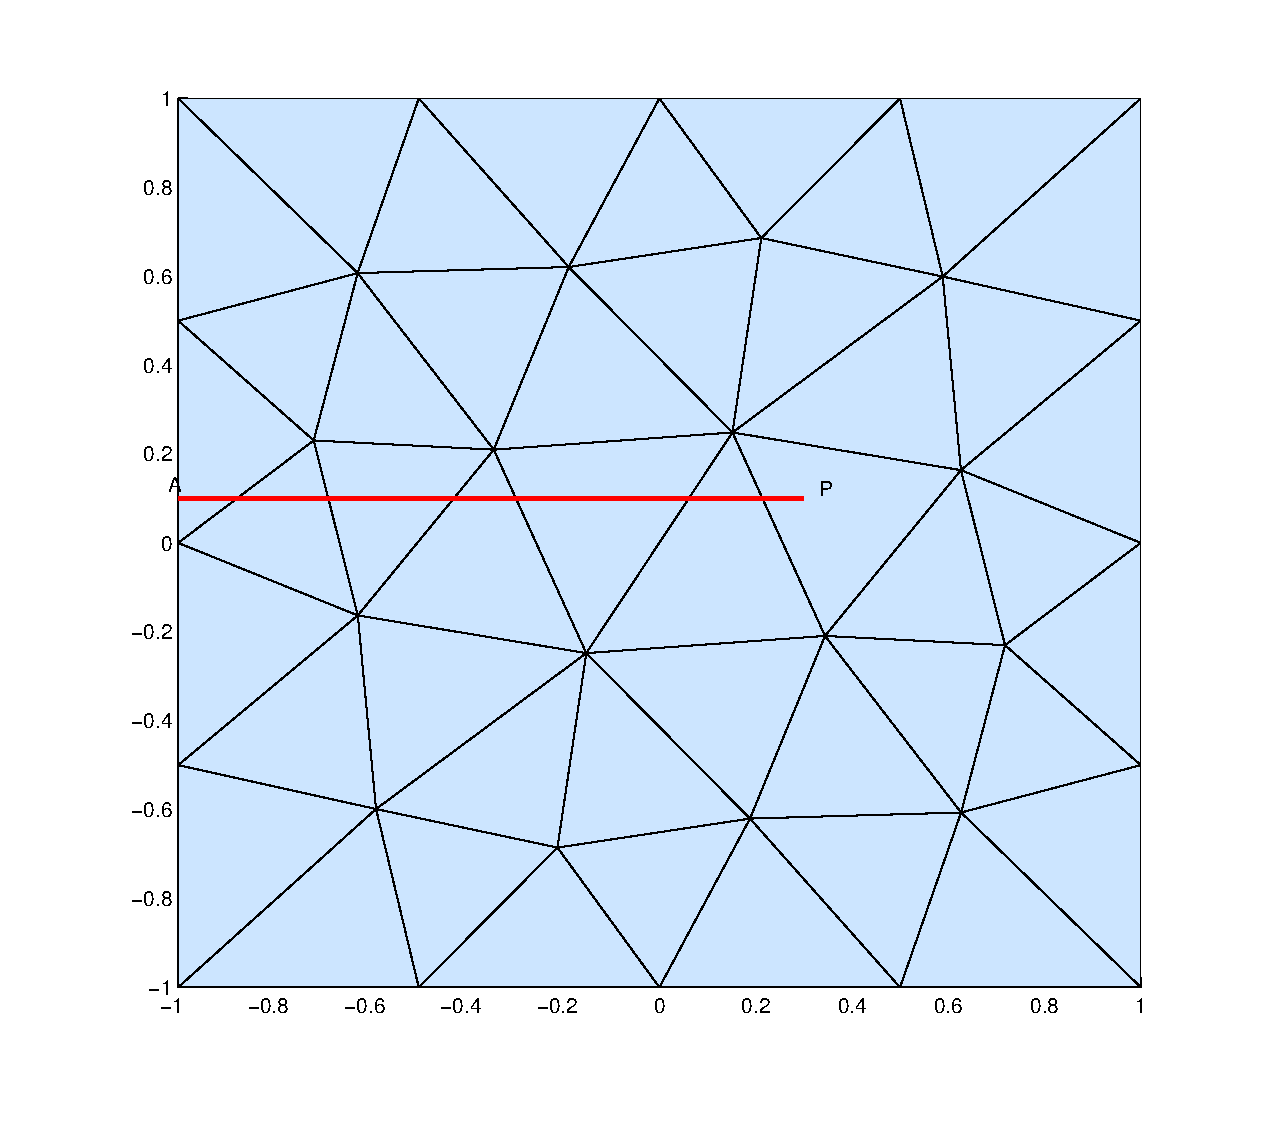
\includegraphics[width=0.5\textwidth]{./pictures/Maxwell05.eps}
\caption{All triangles in $x$ direction affected by one Gauss quadrature point P on triangle $D^k$}
\label{fig1}
\end{figure}
% In Figure \ref{fig1}, the set $A$ includes all of the indexes of elements crossed by the line PA except $k$.

By using (\ref{eq2:2}) and the definition extension of basis functions, we could rewrite the above equation
\begin{equation}
\begin{split}
(\frac{\partial^{\alpha-2}p_h^x}{\partial x^{\alpha-2}},\ell^k(\x))_{D^k}
& \simeq \frac{J^k}{\Gamma(2-\alpha)} \sum_{j=1}^{Q_D} \bigg[\sum_{t\in A}\bigg((\frac{x_j-x_{t-1}}{2})^{2-\alpha}\int_{-1}^{1}(1-\eta)^{1-\alpha}\\
&\cdot(p_h^x)^t(\frac{x_j+x_{t-1}}{2} + \frac{x_j-x_{t-1}}{2}\eta,y_j)d\eta \\
&- (\frac{x_j-x_{t}}{2})^{2-\alpha}\int_{-1}^{1}(1-\eta)^{1-\alpha} \\
&\cdot(p_h^x)^t(\frac{x_j+x_{t}}{2} + \frac{x_j-x_{t}}{2}\eta,y_j)d\eta \bigg)\\
&+ (\frac{x_j-x_{k}}{2})^{2-\alpha}\int_{-1}^{1}(1-\eta)^{1-\alpha} \\
&\cdot(p_h^x)^k(\frac{x_j+x_{k}}{2} + \frac{x_j-x_{k}}{2}\eta,y_j)d\eta ) \bigg]\ \ell^k(\x_j)w_j
\end{split}
\end{equation}
Gauss quadrature with weight function $(1-\eta)^{1-\alpha}$ will be taken in the numerical process.
\begin{rem}
In the process of computation, we must pay enough attention to the fact that there is no link between Lagrange interpolation points and Gauss quadrature points on the triangle.
\end{rem}

Then, we can show a piece of pseudocode for forming the global fractional spatial stiffness matrix.

\begin{algorithm}
\caption{Construct the fractional global spatial stiffness matrix $\widetilde{S}_x$}%\label{alg1}
\begin{algorithmic}[1]
\State \% denote $\pmb{\ell}^k = [\ell_1^k, \ell_2^k, \cdots, \ell_{Np}^k]^T$
\State initialize every block of $\widetilde{S}$ with zero matrix%$\widetilde{S}_{ij}$ is the $i\-th\times j\-th$ block matrix
\For{k = 1:K}
\For{j = 1:$Q_D$}
\State \% $Q_D$ is the total number of Gauss quadrature points
\State find the set A and Xdir of every Gauss point $(x_j^k,y_j^k)$ on triangle $D^k$
\State \% Xdir is a length(A)$\times$2 matrix to store the intervals across by PA on each triangle
\State $(\widetilde{S}_x) _{kk} =  (\widetilde{S}_x) _{kk} + (_{x_{k-1}}D_x^{\alpha-2}\pmb{\ell}^k(\x),\pmb{\ell}^k(\x))_{D^k}$
\For{t=1:length(A)}
\State $(\widetilde{S}_x) _{kt} =  (\widetilde{S}_x) _{kt} + (\frac{1}{\Gamma(2-\alpha)}\int_{x_{t-1}}^{x_t}(x-\xi)^{1-\alpha}\pmb{\ell}^t(\xi,y)d\xi,\pmb{\ell}^k(\x))_{D^k}$
\EndFor
\EndFor
\EndFor
\end{algorithmic}\label{alg1}
\end{algorithm}
\begin{rem}
In Algorithm \ref{alg1}, we only describe the specific procedure of forming the global fractional spatial stiff matrix $\widetilde{S}_x$ for simplicity while
 $\widetilde{S}_y$ can be obtained in the same fashion. In addition, it is unnecessary to store the full global fractional spatial stiffness matrices $\widetilde{S}_x$ and
$\widetilde{S}_y$ for both of them are sparse. The denser the grids are, the sparser the matrices are. Thus, we merely need to store these matrices in the way Matlab does.
\end{rem}

Because of the global property, rather than the local form as usual we recover the global formulation from (\ref{eq3:12}) - (\ref{eq3:14}) as
\begin{eqnarray}
%(\frac{\partial u_h(\x,t)}{\partial t},v)_{D^k} &=& (\nabla \cdot \q_h, v)_{D^k} - (\n\cdot (\q_h - \flux{\q}_h), v)_{\partial D^k}  + (f,v)_{D^k},\\
%(\q_h, \fai)_{D^k} &=& ((\frac{\partial^{\alpha-2}p_h^x}{\partial x^{\alpha-2}},\frac{\partial^{\beta-2}p_h^y}{\partial y^{\beta-2}}), \fai)_{D^k},\\
%(\p_h, \pai)_{D^k} &=& (\nabla u_h, \pai)_{D^k} - (u_h - \flux{u}_h,\n\cdot\pai)_{\partial D^k}.
M \frac{\partial \bm{u}_h}{\partial t} &=& S_x \q_h^x + S_y \q_h^y - \bigcup_{k=1}^K \int_{\partial D^k}\n \cdot ((\q_h^x, \q_h^y) - \flux{\q}_h) \ell(\x) d\bm{s},\\
M \q_h^x &=& \widetilde{S}_x \p_h^x, \quad M \q_h^y = \widetilde{S}_y \p_h^y, \\
M \p_h^x &=& S_x \bm{u}_h - \bigcup_{k=1}^K \int_{\partial D^k} n_x(\bm{u}_h - \flux{\bm{u}}_h) \ell(\x) d\bm{s} \\
M \p_h^y &=& S_y \bm{u}_h - \bigcup_{k=1}^K \int_{\partial D^k} n_y(\bm{u}_h - \flux{\bm{u}}_h) \ell(\x) d\bm{s}
\end{eqnarray}
where $M, S_x, S_y$ are global mass and stiffness matrices and there non-zero diagonal block are constructed by $M^k, S_x^k, S_y^k$ respectively, and $\bigcup_{k=1}^K$
only means composing equations simultaneously for numerical computation.
% and $\bm{u}_h = [\bm{u}_h^1, \bm{u}_h^2, \cdots, \bm{u}_h^K]$,
%$\p_h^x = [(\p^x)_h^1, (\p^x)_h^2, \cdots, (\p^x)_h^K]$, $\p_h^y = [(\p^y)_h^1, (\p^y)_h^2, \cdots, (\p^y)_h^K]$,
%$\q_h^x = [(\q^x)_h^1, (\q^x)_h^2, \cdots, (\q^x)_h^K]$, $\q_h^y = [(\q^y)_h^1, (\q^y)_h^2, \cdots, (\q^y)_h^K]$.

\section{Stability analysis and error estimates}
Before approaching theoretical analysis, we need to introduce the following result:
\begin{lem}
Assume that $\Omega$ has been triangulated into $K$ elements, $D^k$, then
\begin{equation}
\sum_{k=1}^{K} (\n\cdot\textbf{\emph{u}}, v)_{\partial D^k} = \oint_{\Gamma}\{\textbf{\emph{u}}\}\cdot [v] ds + \oint_{\Gamma_i}\{v\}[\textbf{\emph{u}}]ds.
\end{equation}
\end{lem}
The proof is easy by rewriting and then summing the averages and jumps of all the terms  along one edge.

By using the above Lemma and summing all the terms of (\ref{eq3:9}) - (\ref{eq3:11}), we can obtain the primal formulation:
Find $(u_h,\p_h,\q_h) \in H^1(0,T;V_h)\times (L^2(0,T;V_h))^2\times (L^2(0,T;V_h))^2$ such that
for all $(v,\fai,\pai) \in H^1(0,T;V_h)\times (L^2(0,T;V_h))^2\times (L^2(0,T;V_h))^2$ the following holds
\begin{equation}
B(u_h,\p_h,\q_h;v,\fai,\pai) = \mathcal{L}(v,\fai,\pai).
\end{equation}
Denote $(\cdot,\cdot) = (\cdot,\cdot)_{\Omega}$ if it causes no misunderstanding. Let us remind the facts that the numerical flux is single valued and the homogeneous boundary condition,
 %and $(u_h(\cdot,0),v(\cdot,0)) = u(\cdot,0),v(\cdot,0))$
then the discrete bilinear form $B$ can be defined as
\begin{equation}
\begin{split}
B(u_h,\p_h,\q_h;v,\fai,\pai)
& :=  \int_{0}^{T}(\frac{\partial u_h}{\partial t},v) dt  + \int_{0}^{T}(\q_h,\nabla v)dt\\
& + \int_{0}^{T} (\q_h,\fai)dt - \int_{0}^{T}\big((\frac{\partial^{\alpha-2}p_h^x}{\partial x^{\alpha-2}},\frac{\partial^{\beta-2}p_h^y}{\partial y^{\beta-2}}),\fai \big)dt \\
& + \int_{0}^{T} (\p_h,\pai)dt + \int_{0}^{T}(u_h,\nabla\cdot\pai)dt\\
& - \int_{0}^{T} ( \oint_{\Gamma}\flux{\q}_h\cdot[v]ds + \oint_{\Gamma_i}\flux{u}_h[\pai] ds )dt.
\end{split}
\label{eq4:3}
\end{equation}
The discrete linear form $\mathcal{L}$ is given by
\begin{equation}
\mathcal{L}(u_h,\p_h,\q_h;v,\fai,\pai) = \int_{0}^{T}(f,v)dt.
\end{equation}
Provided that the numerical fluxes $\flux{u}_h, \flux{\q}_h$ are consistent, the primal formulation (\ref{eq4:3}) is consistent, which implies that the exact solution $(u,\p,\q)$ of (\ref{eq3:2}) satisfies
\begin{equation}
B(u,\p,\q;v,\fai,\pai) = \mathcal{L}(v,\fai,\pai).\label{eq4:5}
\end{equation}
for all $(v,\fai,\pai) \in H^1(0,T;V_h)\times (L^2(0,T;V_h))^2\times (L^2(0,T;V_h))^2$.
\subsection{Numerical ability}
Let $(\widetilde{u}_h,\widetilde{\p}_h,\widetilde{\q}_h) \in H^1(0,T;V_h)\times (L^2(0,T;V_h))^2\times (L^2(0,T;V_h))^2$ be the approximation of solution
$(u_h,\p_h,\q_h)$.We denote $e_{u_h} := u_h - \widetilde{u}_h$, $e_{\p_h} := \p_h - \widetilde{\p_h}$ and $e_{\q_h} := \q_h - \widetilde{\q}_h$ as the perturbation errors.
\begin{thm}{($L^2$ stability).}
Numerical scheme (\ref{eq4:5}) is $L^2$ stable, and for all $t\in (0,T)$ its solution satisfies
\begin{equation}
\begin{split}
&\parallel e_{u_h}(\cdot,t)\parallel^2_{L^2(\Omega)} \ = \ \parallel e_{u_h}(\cdot,0)\parallel^2_{L^2(\Omega)} \\
& - \ 2cos((\alpha/2-1)\pi)\int_{0}^{t} \int_{c}^{d}\parallel e_{p_h^x}(\cdot,y,t) \parallel^2_{L^2(a,b)} dydt\\
& - \ 2cos((\beta/2-1)\pi) \int_{0}^{t} \int_{a}^{b}\parallel e_{p_h^y}(x,\cdot,t) \parallel^2_{L^2(c,d)} dxdt.
\end{split}
\end{equation}
\label{thm1}
\end{thm}
\begin{proof}
We just prove the case $t = T$. From (\ref{eq4:3}), we recover the perturbation equation
\begin{equation}
B(e_{u_h},e_{\p_h},e_{\q_h};v,\fai,\pai) = 0
\end{equation}
for all $(v,\fai,\pai) \in H^1(0,T;V_h)\times (L^2(0,T;V_h))^2\times (L^2(0,T;V_h))^2$. Take $v = e_{u_h}$, $\fai = - e_{\p_h}$, and
$\pai = e_{\q_h}$, we obtain
\begin{equation}
\begin{split}
0 &= B(e_{u_h},e_{\p_h},e_{\q_h};e_{u_h},-e_{\p_h},e_{\q_h}) \\
&= \frac{1}{2}\int_{0}^{T} \frac{\partial }{\partial t} \parallel e_{u_h}(\cdot,t)\parallel^2_{L^2(\Omega)} dt + \int_{0}^{T} \int_{\Omega}\nabla\cdot (e_{u_h}e_{\q_h})d\x dt \\
& + \ 2cos((\alpha/2-1)\pi)\int_{0}^{T} \int_{c}^{d}\parallel e_{p_h^x}(\cdot,y,t) \parallel^2_{L^2(a,b)} dydt\\
& + \ 2cos((\beta/2-1)\pi) \int_{0}^{T} \int_{a}^{b}\parallel e_{p_h^y}(x,\cdot,t) \parallel^2_{L^2(c,d)} dxdt\\
& - \int_{0}^{T}(\oint_{\Gamma}\flux{e}_{\q_h}\cdot[e_{u_h}]ds + \oint_{\Gamma_i}\flux{e}_{u_h}[e_{\q_h}]ds)dt.
\end{split}
\label{eq4:8}
\end{equation}
In the above Eq (\ref{eq4:8}) through integration by parts,
\begin{equation}
\begin{split}
\int_{\Omega_h}\nabla\cdot(e_{u_h}e_{\q_h})d\x  & = \sum_{k=1}^{K}\int_{D^k}\nabla\cdot(e_{u_h}e_{\q_h})d\x
= \sum_{k=1}^{K}\oint_{\partial D^k}\n\cdot e_{\q_h}e_{u_h}ds\\%(e_{u_h}^- = 0 on \Gamma_b)
&= \oint_{\Gamma_i}(\n^+\cdot e_{\q_h}^+e_{u_h}^+ + \n^-\cdot e_{\q_h}^- e_{u_h}^-)ds + \oint_{\Gamma_b} \n \cdot e_{\q_h} e_{u_h} ds.
\end{split}\label{eq4:9}
\end{equation}
and when $\flux{e}_{u_h} = e_{u_h}^+$, $\flux{e}_{\q_h} = e_{\q_h}^-$ (or $\flux{e}_{u_h} = e_{u_h}^-$, $\flux{e}_{\q_h} = e_{\q_h}^+$),
Beside, with $e^-_{u_h} = 0$ on the external boundary $\Gamma_b$, when $\flux{e}_{u_h} = e_{u_h}^+$, $\flux{e}_{\q_h} = e_{\q_h}^-$,
\begin{equation}
\begin{split}
& \oint_{\Gamma}\flux{e}_{\q_h}\cdot[e_{u_h}]ds + \oint_{\Gamma_i}\flux{e}_{u_h}[e_{\q_h}]ds \\
&= \oint_{\Gamma_i}(\n^+\cdot e_{\q_h}^+e_{u_h}^+ + \n^-\cdot e_{\q_h}^- e_{u_h}^-)ds + \oint_{\Gamma_b} \n \cdot e_{\q_h} e_{u_h} ds.
\end{split}\label{eq4:10}
\end{equation}

Combining (\ref{eq4:9})-(\ref{eq4:10}), the desired result is obtained.
\end{proof}
\subsection{Error estimate}
For the error estimate, we need to define several orthogonal projection operators, $\mathbb{P}: H^1(\Omega_h)\rightarrow V_h$ and $\mathbb{S}: H^1(\Omega_h)\times H^1(\Omega_h)\rightarrow V_h\times V_h$. For all the elements, $D^k,$ $k= 1,2,\cdots,K$,
$\mathbb{P}, \mathbb{S}$ are defined to satisfy
\begin{equation}
(\mathbb{P}u-u,v)_{D^k} = 0, \quad \forall v\in V_h,
\end{equation}
and
\begin{equation}
(\mathbb{S}\mathbf{w} - \mathbf{w}, \fai)_{D^k} = 0, \quad \forall\fai \in V_h\times V_h.
\end{equation}


\begin{thm}
The error of our numerical scheme with flux applied model satisfies
\begin{equation}
\parallel u(\x,t) - u_h(\x,t) \parallel_{L^2(\Omega_h)} \leqslant c(\alpha,\beta)h^{N+1}, \quad \alpha, \beta\in(1,2),
\end{equation}
where $c(\alpha,\beta)$ is independent of h.
\end{thm}
\begin{proof}
We denote
$$ e_u = u(\x,t) - u_h(\x,t), \ e_{\p}(\x,t) = \p(\x,t) - \p_h(\x,t), \ e_\q = \q(\x,t) - \q_h(\x,t),$$
then recover the error equation
\begin{equation}
B(e_u,e_\p,e_\q;v,\fai,\pai) = 0 \label{eq4:14}
\end{equation}
for all $(v,\fai,\pai) \in H^1(0,T;V_h)\times (L^2(0,T;V_h))^2\times (L^2(0,T;V_h))^2$.
Take $$ v = \mathbb{P}u - u_h,\ \fai = \p_h - \mathbb{S}\p,\ \pai = \mathbb{S}\q - \q_h$$
in the (\ref{eq4:14}). After rearranging terms, we obtain
\begin{equation}
B(v,-\fai,\pai;v,\fai,\pai) = B(v^e,-\fai^e,\pai^e;v,\fai,\pai) \label{eq4:15}
\end{equation}
where $v^e, \bm{w}^e$ and $\bm{z}^e$ are given as
$$v^e = \mathbb{P}u - u, \fai^e = \p - \mathbb{S}\p, \pai^e = \mathbb{S}\q - \q.$$
Following the discussion in the proof of Theorem (\ref{thm1}) the left side of (\ref{eq4:15}) becomes
\begin{equation}
\begin{split}
& B(v,-\fai,\pai;v,\fai,\pai) = \frac{1}{2}\int_{0}^T\frac{\partial}{\partial t}\parallel v(\cdot,t)\parallel^2_{L^2(\Omega_h)}dt \\
& + cos((\alpha/2-1)\pi)\int_0^T\int_{c}^{d}\parallel \phi^x(\cdot,y,t)\parallel^2_{H^{\frac{\alpha}{2}-1}{(a,b)}}dydt\\
& + cos((\beta/2-1)\pi)\int_0^T\int_{a}^{b}\parallel \phi^y(x,\cdot,t)\parallel^2_{H^{\frac{\beta}{2}-1}{(c,d)}}dxdt,
\end{split}
\end{equation}
and the right hand can be expressed as
\begin{equation}
B(v^e,-\fai^e,\pai^e;v,\fai,\pai) = \Rmnum{1} + \Rmnum{2} + \Rmnum{3} + \Rmnum{4},
\end{equation}
where
\begin{equation}
\Rmnum{1} = \int_0^T(\frac{\partial v^e(\cdot,t)}{\partial t}, v(\cdot,t))dt,
\end{equation}
\begin{equation}
\Rmnum{2} = \int_0^T\big[(\pai^e,\nabla v) + (v^e, \nabla\cdot\pai) + (\pai^e, \fai) -(\fai^e, \pai) \big]dt
\end{equation}
\begin{equation}
\Rmnum{3} = -\int_{0}^{T} \big( \int_{\Gamma}\flux{\pai}^e\cdot[v] ds + \int_{\Gamma_i}v^e \ [\pai] ds \big) dt.
\end{equation}
\begin{equation}
\Rmnum{4} =  \int_0^T\big[   (\frac{\partial^{\alpha-2}{\phi^e}^x }{\partial x^{\alpha-2}},\phi^x)  + (\frac{\partial^{\beta-2}{\phi^e}^y }{\partial y^{\beta-2}},\phi^y) \big]dt.
\end{equation}
Using Cauchy-Schwarz inequality and the standard approximation theory, we obtain
\begin{equation}
\begin{split}
\Rmnum{1} &= \frac{1}{2}\int_0^T\parallel \frac{\partial v^e(\cdot,t)}{\partial t} \parallel^2_{L^2(\Omega_h)} dt + \frac{1}{2}\int_0^T \parallel v(\cdot,t)\parallel_{L^2(\Omega_h)} dt \\
&\leqslant ch^{2N+2} + \frac{1}{2}\int_0^T\parallel v(\cdot,t) \parallel^2_{L^2(\Omega)}dt
\end{split}
\end{equation}
where c is a constant.
In $\Rmnum{2}$, all terms vanish because of Galerkin orthogonality.
To deal with the term $\Rmnum{3}$, let us reexamine the construction of our Lagrange interpolation bases.
In our scheme, we require the same number of Lagrange interpolation points on every element, thus the basis functions of both elements are equal along the internal edge $e \in \Gamma_i$. On the external edge $\Gamma_b$, it is also the same case due to the imposed boundary conditions. Thus for any basis function $v$ we have $[v]=0$ on all edges, from which the terms in $\Rmnum{3}$ vanish.
As for $\Rmnum{4}$, by using Young's inequality, we could obtain
\begin{equation}
\begin{split}
\Rmnum{4} &\leqslant \int_0^T \bigg( \frac{\varepsilon_1}{2}\parallel \pai^e(\cdot,t)\parallel^2_{L^2(\Omega_h)} + \frac{1}{2\varepsilon_2}\parallel\fai(\cdot,t)\parallel^2_{\Omega_h} \\
&+ \frac{\varepsilon_2}{2}\parallel {\phi^e}^x(\cdot,t) \parallel^2_{L^2(\Omega_h)} + \frac{1}{2\varepsilon_2}\int_c^d\parallel\phi^x(\cdot,y,t)\parallel^2_{H^{\alpha-2}(a,b)}dy\\
&+\frac{\varepsilon_3}{2}\parallel{\phi^e}^y(\cdot,t)\parallel^2_{L^2(\Omega_h)}
 \int_a^b\parallel\phi^y(x,\cdot,t)\parallel^2_{H^{\beta-2}(c,d)}dx\bigg )dt\\
&\leqslant c/\varepsilon h^{2N+2} + c\varepsilon \big( \int_0^T\int_c^d\parallel\phi^x(\cdot,y,t)\parallel^2_{H^{\frac{\alpha}{2}-1}(a,b)}dy\\
 &+ \int_a^b\parallel\phi^y(x,\cdot,t)\parallel^2_{H^{\frac{\beta}{2}}(c,d)}dx dt\big)
\end{split}
\end{equation}
where $\varepsilon_1,\varepsilon_2, \varepsilon_3$ are small numbers to control the equality and $\varepsilon = max(\varepsilon_1,\varepsilon_2,\varepsilon_3)$. Combining all the above estimates,
\begin{equation}
\begin{split}
&\frac{1}{2}\parallel v(\cdot,T)\parallel^2_{L^2(\Omega_h)}\\
&+ (cos((\alpha/2-1)\pi)-c\varepsilon)\int_0^T \int_c^d\parallel\phi^x(\cdot,y,t)\parallel^2_{H^{\frac{\alpha}{2}-1}(a,b)}dydt  \\
&+ (cos((\beta/2-1)\pi)-c\varepsilon)\int_{0}^T\int_c^d\parallel\phi^y(x,\cdot,t)\parallel^2_{H^{\frac{\beta}{2}-1}(c,d)} dxdt \\
&\leqslant (c/\varepsilon)h^{2N+2} + c\int_0^T\parallel v(\cdot,t)\parallel^2_{L^2(\Omega_h)}dt.
\end{split}
\end{equation}
According to Gr\"{o}nwall's lemma and the standard approximation theory, the desired result is obtained.

\end{proof}
\section{Numerical results}
In this section, we will provide some numerical examples to validate analysis. To deal with the method-of-line fractional PDE, i.e., the classical ODE system, we utilize the low-storage five stage fourth order explicit Runge-Kutta method. To ensure the overall error is dominated by space error, small time steps are used.

We consider the problem
\begin{equation}
\frac{\partial u(x,y,t)}{\partial t} = \frac{\partial ^{\alpha}u(x,y,t)}{\partial x^{\alpha}} + \frac{\partial ^{\beta}u(x,y,t)}{\partial y^{\beta}} + f(x,y,t)
\end{equation}
where
\begin{displaymath}
\begin{split}
f(x,y,t)
&= -e^{-t}\big((x^2-1)^3(y^2-1)^3 - (y^2-1)^3_{-1}D_x^{\alpha-2}(6(x^2-1)(5x^2-1))\\
&- (x^2-1)^3_{-1}D_y^{\beta-2}(6(y^2-1)(5y^2-1))\big)
\end{split}
\end{displaymath}
on the computational domain $\Omega=(-1,1)\times(-1,1)$ and $\alpha, \beta \in (1,2)$.
We consider the initial condition
\begin{equation}
u(x,y,0) = (x^2-1)^3(y^2-1)^3
\end{equation}
and the Dirichlet condition
\begin{equation}
u(x,y,t) = 0, \quad (x,y) \in \partial \Omega.
\end{equation}
The exact solution is $u(x,y,t)=e^{-t}(x^2-1)^3(y^2-1)^3$.

%Two kinds of meshes including regular and irregular grids are utilized in our example, shown in Figure \ref{fig2} and \ref{fig3} respectively.

\begin{table}
\centering
\caption{Numerical errors ($L_2$) and order of convergence on regular meshes at T=0.001. N denotes the order of polynomial in two variables, and K is the total number of triangle elements.}
    \begin{tabular}{*{11}{|c}|}
      \hline
      &K & \multicolumn{1}{c|}{18} & \multicolumn{2}{c|}{32} & \multicolumn{2}{c|}{72} & \multicolumn{2}{c|}{128}  \\
    \hline
     N &$(\alpha,\beta)$ &  error  &  error & order &  error & order &  error & order   \\ \hline
     \multirow{4}{*}{1} & (1.01,1.01)  &2.76e-1 &1.61e-1 &1.87 &7.43e-2 &1.91 &4.28e-2 &1.92 \\
                    \cline{2-9}
                    & (1.9,1.1) & 2.75e-1 &1.60e-1 &1.88 &7.37e-2 &1.91 &5.49e-2 &1.91 \\
                    \cline{2-9}
                    & (1.5,1.5) &2.76e-1 &1.60e-1 &1.90 &7.41e-2 &1.90 &4.26e-2 &1.92 \\
                    \cline{2-9}
                    %& (1.1,1.9) &2.75e-1 &1.60e-1 & &7.37e-2 & &5.46e-2 & \\
                    %\cline{2-9}
                    & (1.99,1.99) &2.75e-1 &1.60e-1 &1.88 &7.31e-2 &1.93 &4.21e-2 &1.92 \\
                    \hline
     \multirow{4}{*}{2} & (1.01,1.01)  &4.12e-2 &2.06e-2 &2.41 &7.18e-3 &2.60 &3.22e-3 &2.79 \\
                    \cline{2-9}
                    & (1.9,1.1) & 4.05e-2&1.99e-2 &2.47 &6.68e-3 &2.69 &4.28e-3 &2.89 \\
                    \cline{2-9}
                    & (1.5,1.5) &4.09e-2 &2.02e-2 &2.45 &6.93e-3 &2.64 &3.06e-3 &2.84 \\
                    \cline{2-9}
                  %  & (1.1,1.9) &4.05e-2 &2.00e-2 & &6.68e-3 & &4.48e-3 & \\
                    \cline{2-9}
                    & (1.99,1.99) &3.97e-2 &1.92e-2 &2.53 &6.10e-3 &2.83 &2.46e-3 &3.16 \\
                    \hline
     \multirow{4}{*}{3} & (1.01,1.01)  &1.29e-2 &4.65e-3 &3.55 &1.02e-3 &3.74 &3.37e-4 &3.85 \\
                    \cline{2-9}
                    & (1.9,1.1) &1.20e-2 &4.21e-3 &3.64 &8.95e-4 &3.82 &2.94e-4 &3.87 \\
                    \cline{2-9}
                    & (1.5,1.5) &1.25e-2  &4.45e-3 &3.59 &9.59e-4 &3.79 &3.12e-4 &3.90 \\
                    \cline{2-9}
                    %& (1.1,1.9) &1.20e-1 &4.21e-3 & &8.95e-4 & &4.92e-4 & \\
                    \cline{2-9}
                    & (1.9,1.9) &1.12e-2 &3.78e-3 &3.78 &7.79e-4 &3.90 &2.62e-4 &3.78 \\
                    \hline
    \end{tabular}
    \label{table1}
\end{table}


\begin{table}
\centering
\caption{Numerical errors ($L_2$) and order of convergence on irregular meshes at T=0.001. N denotes the order of polynomial in two variables, and K is the total number of triangle elements.}
    \begin{tabular}{*{9}{|c}|}
      \hline
      &K & \multicolumn{1}{c|}{8} & \multicolumn{2}{c|}{46} & \multicolumn{2}{c|}{97} & \multicolumn{2}{c|}{146} \\
    \hline
     N &$(\alpha,\beta)$ &  error  &  error & order &  error & order &  error & order   \\ \hline
     \multirow{4}{*}{1} & (1.01,1.01)  &2.90e-1 &1.16e-1 &1.05 &5.67e-2 &1.92 &3.80e-2 &1.96 \\
                    \cline{2-9}
                    & (1.1,1.9) & 2.90e-1&1.15e-1 &1.06 &5.62e-2 &1.92 &3.77e-2 &1.95 \\
                    \cline{2-9}
                    & (1.5,1.5) &2.91e-1 &1.15e-1 &1.05 &5.65e-2 &1.91 &3.78e-2 &1.97 \\
                    \cline{2-9}
                  %  & (1.1,1.9) & & & & & & & \\
                    \cline{2-9}
                    & (1.99,1.99) &2.89e-1 &1.14e-1 &1.06 &5.57e-2 &1.92 &3.74e-2 &1.95 \\
                    \hline
     \multirow{4}{*}{2} & (1.01,1.01) &1.62e-1 &1.08e-2 &3.10 &4.50e-3 &2.35 &2.42e-3 &3.03 \\
                    \cline{2-9}
                    & (1.1,1.9) &1.62e-1 &1.03e-2 &3.15 &4.06e-3 &2.50 &2.13e-3 &3.16 \\
                    \cline{2-9}
                    & (1.5,1.5) &1.62e-1 &1.05e-2 &3.13 &4.30e-3 &2.39 &2.27e-3 &3.12 \\
                    \cline{2-9}
                    %& (1.1,1.9) & & & & & & & \\
                    \cline{2-9}
                    & (1.99,1.99) &1.62e-1 &9.69e-3 &3.22 &3.62e-3 &2.64 &1.82e-3 &3.36 \\
                    \hline
     \multirow{4}{*}{3} & (1.01,1.01) &4.07e-2 &1.56e-3 &3.73 &5.65e-4 &2.72 &1.86e-4 &5.43 \\
                    \cline{2-9}
                    & (1.1,1.9) &4.02e-2 &1.41e-3 &3.83 &4.80e-4 &2.89 &1.64e-4 &5.25 \\
                    \cline{2-9}
                    & (1.5,1.5) &4.05e-2 &1.49e-3 &3.78 &5.29e-4 &2.78 &1.79e-4 &5.30 \\
                    \cline{2-9}
                    %& (1.1,1.9) & & & & & & & \\
                    \cline{2-9}
                    & (1.9,1.9) &3.98e-2 &1.29e-3 &3.92 &4.27e-4 &2.96 &1.54e-4 &4.99 \\
                    \hline
    \end{tabular}
    \label{table2}
\end{table}


We first give the numerical results of above example on regular meshes and the
rate of convergence is computed using the sequence of regular nested refined meshes.
In Table \ref{table1} and \ref{table2}, we note a convergence rate very close to $\mathcal{O}(h^{N+1})$, which demonstrates that LDG is generally optimal for the two-dimensional case. Figure \ref{fig2} shows the the convergence rate which is optional on regular meshes with $\alpha = \beta = 1.5$ and $\alpha = 1.1, \beta = 1.9$ respectively.
Note that the small deviations from the optimal order are caused by the unstructured nature of the grid and numerical quadrature for fractional integral operators.

\begin{figure}
\centering
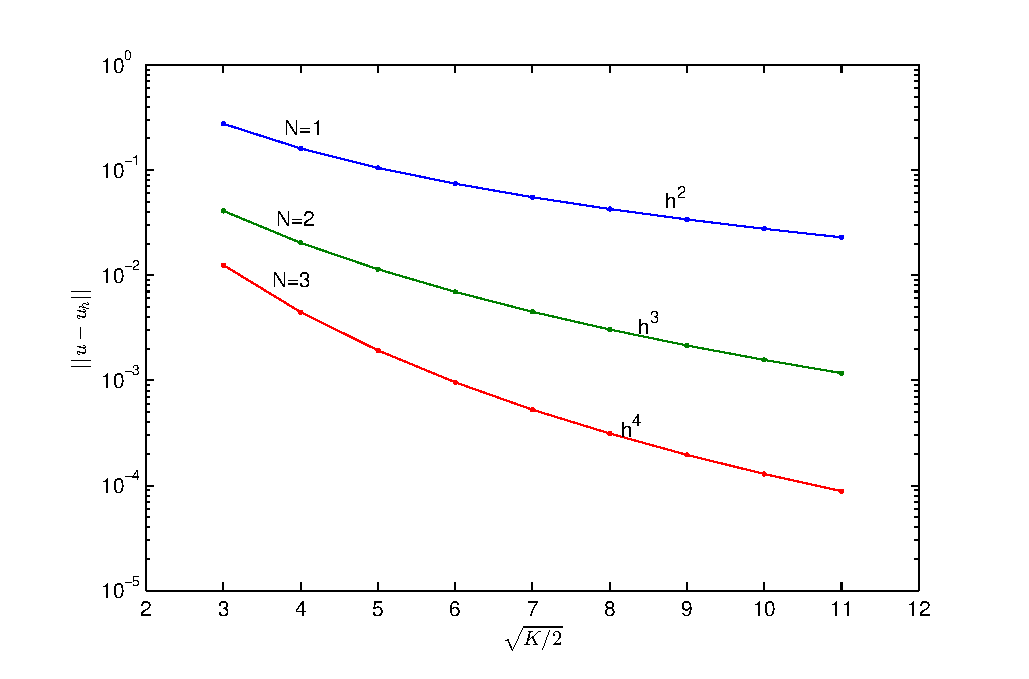
\includegraphics[width=0.45\textwidth]{./pictures/1.5&1.5.eps}
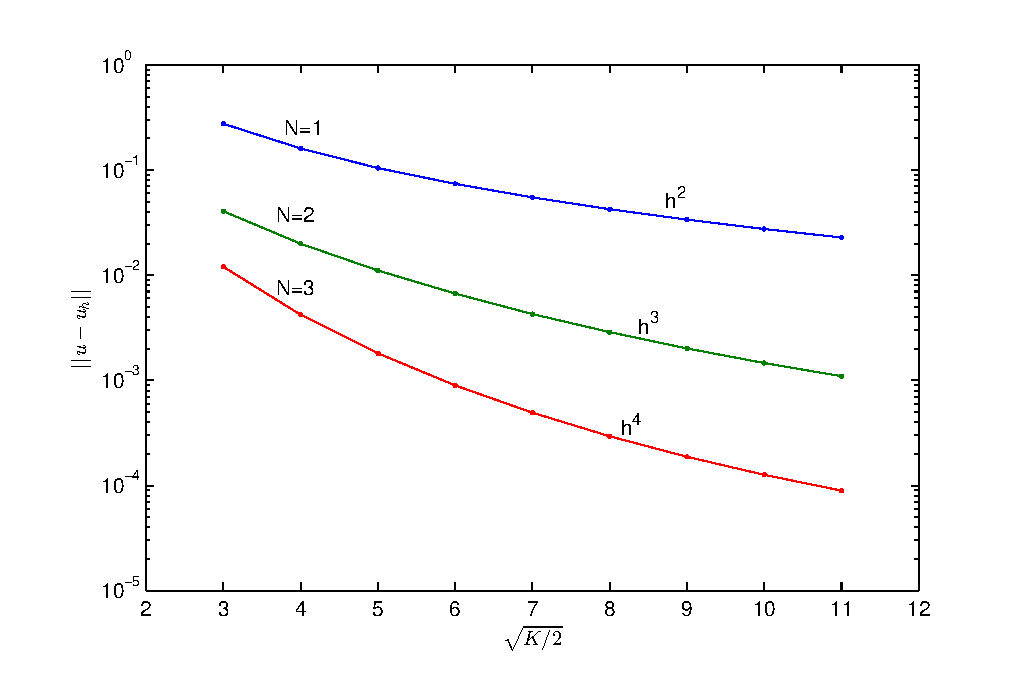
\includegraphics[width=0.45\textwidth]{./pictures/1.1&1.9.eps}
\caption{On the left we show the convergence rate for the fractional diffusion equation using LDG with regular meshes when $\alpha = \beta = 1.5$, while the right shows the results obtained by $\alpha =1.1, \beta = 1.9.$}
\label{fig2}
\end{figure}

\section{Conclusions}
In this paper, we succeed to develop local nodal discontinuous Galerkin methods for two dimensional \RL fractional equations over  unstructured meshes, and give stability analysis and error estimates. Numerical experiments confirm that the optional convergence order can be obtained by choosing appropriate flux. For the convenience of theoretical analysis and easily construct numerical examples, we restrict our models to the homogeneous boundary conditions. Actually, there is no need to require special Direchlet conditions when dealing with Caputo fractional diffusion equations as \cite{xia} shows. Further, we need to note that the Algorithm \ref{alg1} show in section 3 for forming global fractional stiffness matrix is a simple but efficient way, even for high-performance computing. 



%\begin{figure}
%\centering
%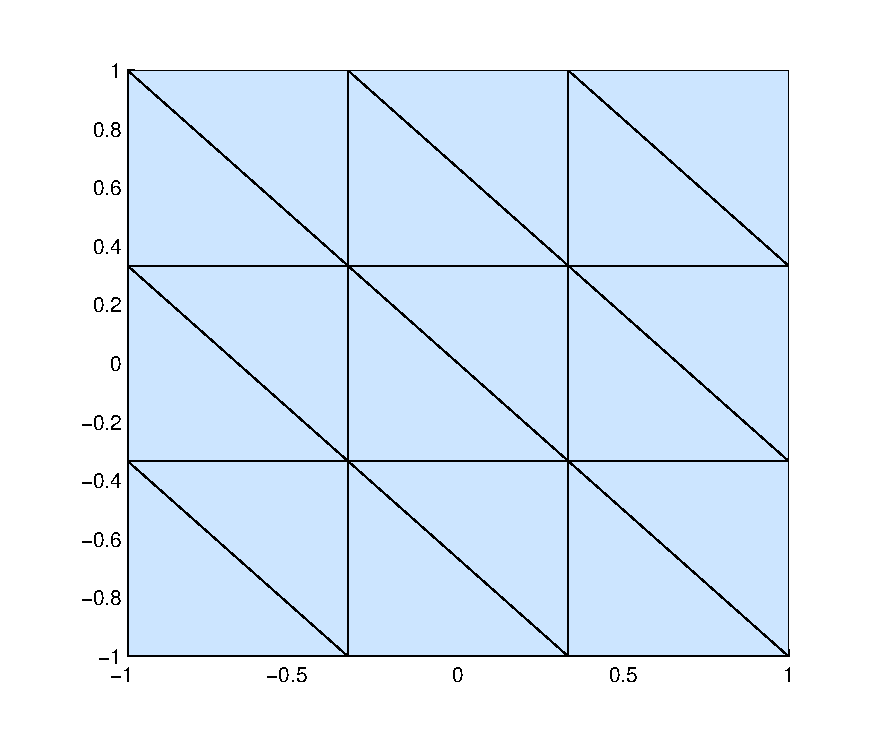
\includegraphics[width=0.3\textwidth]{./pictures/regular18.eps}
%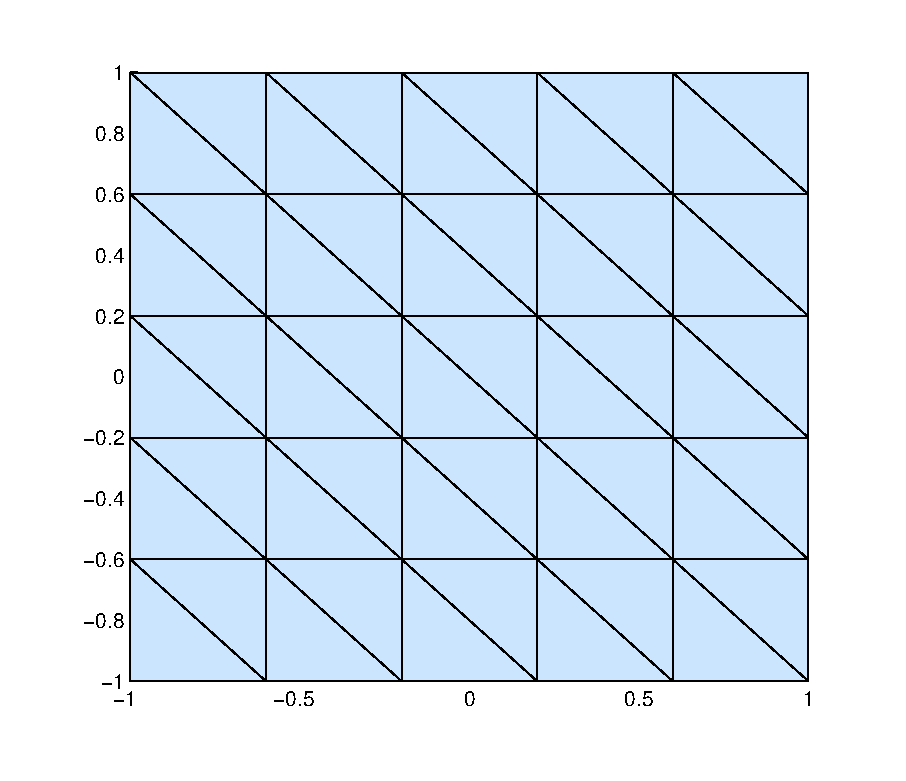
\includegraphics[width=0.3\textwidth]{./pictures/regular50.eps}
%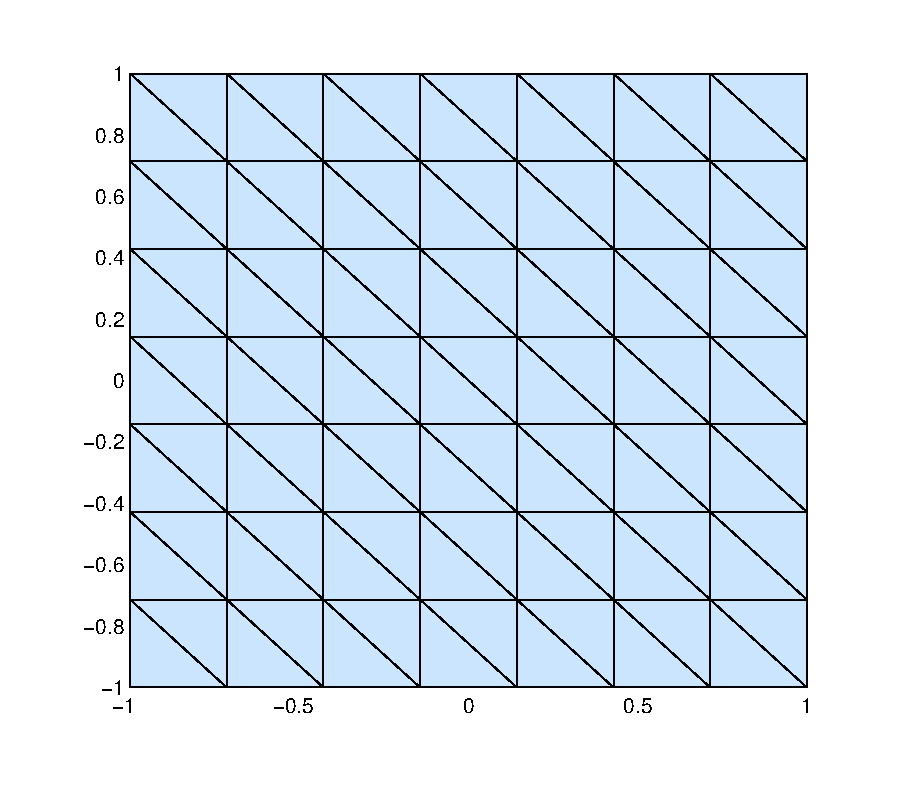
\includegraphics[width=0.3\textwidth]{./pictures/regular98.eps}
%\caption{ Sequence of three regular meshes used to perform convergence analysis.}
%\label{fig2}
%\end{figure}
%
%\begin{figure}
%\centering
%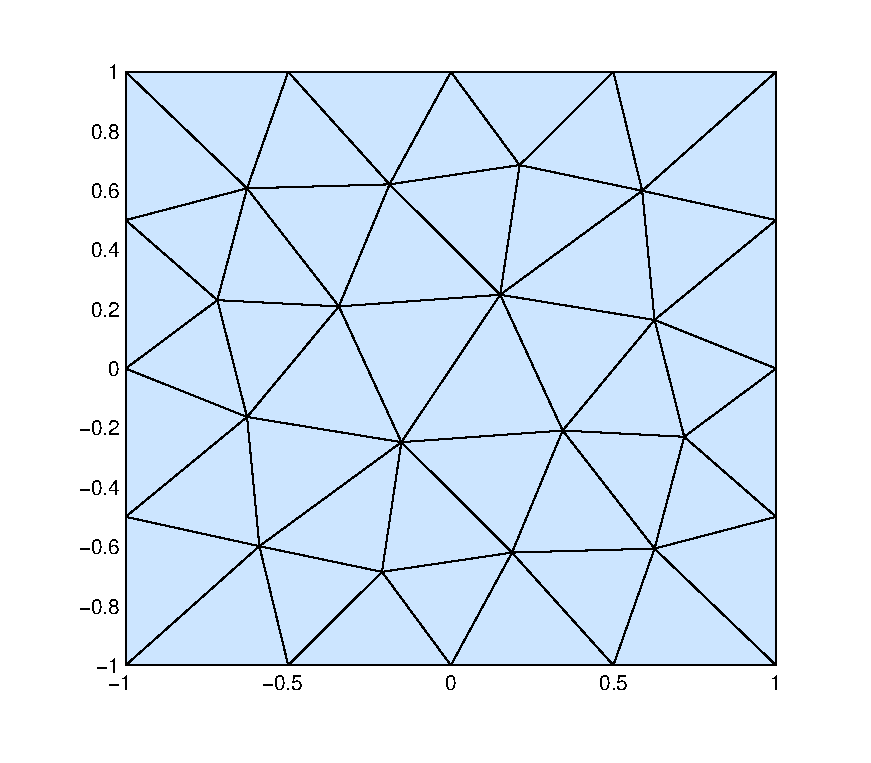
\includegraphics[width=0.3\textwidth]{./pictures/unregular46.eps}
%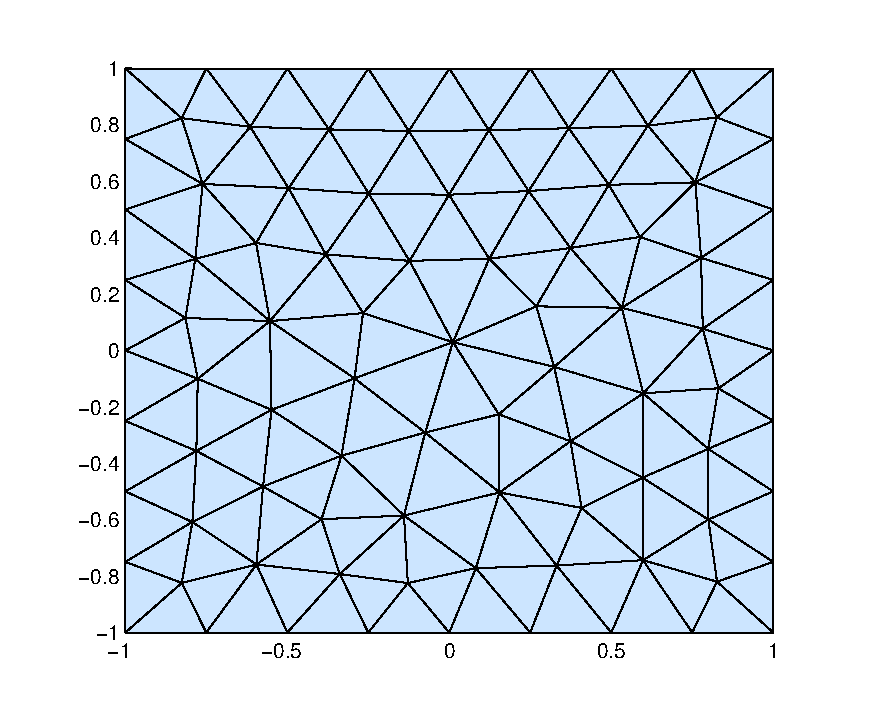
\includegraphics[width=0.3\textwidth]{./pictures/unregular97.eps}
%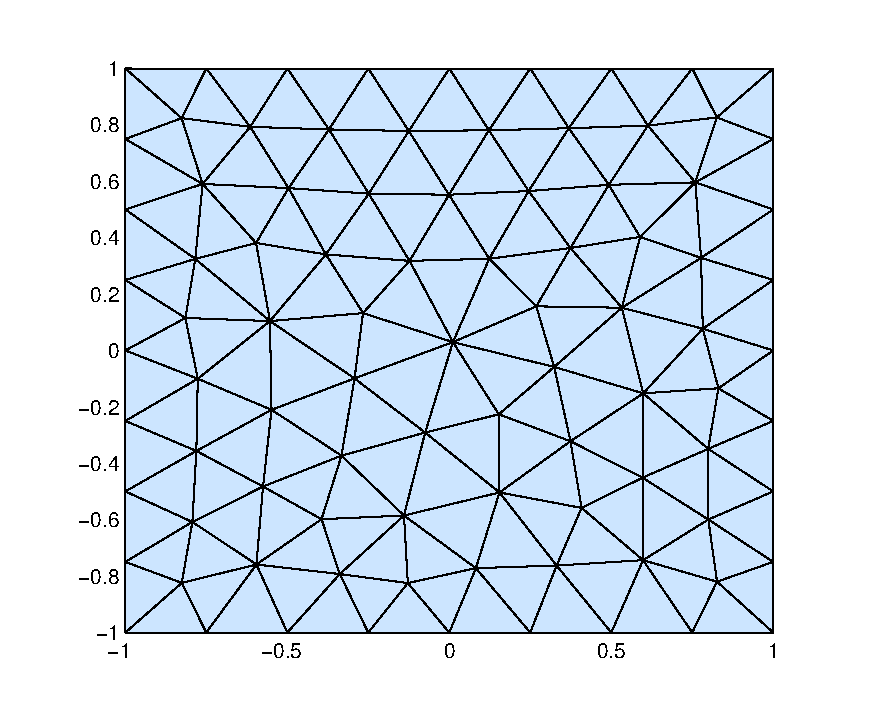
\includegraphics[width=0.3\textwidth]{./pictures/unregular146.eps}
%\caption{ Sequence of three irregular meshes used to perform convergence analysis.}
%\label{fig3}
%\end{figure}

\newpage
\begin{thebibliography}{100}
\bibitem{Adams:1975}
R.~A. Adams. Sobolev Spaces. Academic Press, New York, 1975.

\bibitem{Podlubny:1999}
I.~Podlubny, Fractional Differential Equations, Academic Press, New York,
  1999.

\bibitem{samko}
S.~G. Samko, A.~A. Kilbas, and O.~I. Marichev. Fractional Integrals and Derivatives: Theory and
Applications. Gordon and Breach, New York, 1993.

\bibitem{canuto}
Canuto C, Hussaini M, Quarteroni A and Zang T (2006) Spectral Methods. Scientific Computation,
Springer-Verlag, Berlin, fundamentals in single domains.

\bibitem{chen1}
Chen Q, Babu\v{s}ka I. Approximate optimal points for polynomial interpolation of real functions in an interval and in a triangle[J]. Computer Methods in Applied Mechanics and Engineering, 1995, 128(3): 405-417.

\bibitem{jan1}
Hesthaven J S, Warburton T. Nodal discontinuous Galerkin methods: algorithms, analysis, and applications[M]. Springer, 2008.

%\bibitem{jan2}
%J.S. Hesthaven, From electrostatics to almost optional nodal sets for polynomial interpolation in simplex, SIAM J.Numer. Anal. 35(1988), pp. 655-676.
%
\bibitem{jan2}
Hesthaven J S. From electrostatics to almost optimal nodal sets for polynomial interpolation in a simplex[J]. SIAM Journal on Numerical Analysis, 1998, 35(2): 655-676.

\bibitem{meer}
M. M. Meerschaert, C. Tadjeran, Finite difference approximations for fractional advection-dispersion
flow equations, J. Comput. Appl. Math. 172 (2004) 65-77

\bibitem{tian1}
W. Y. Tian, H. Zhou, W. H. Deng, A class of second order difference approximation for solving space
fractional diffusion equations, submitted. arXiv:1201.5949 [math.NA]

\bibitem{Ervin:2006}
V.~J. Ervin, J.~E. Roop, Variational formulation for the stationary fractional
  advection dispersion equation, Numer. Methods Partial Differential Eq. 22~(3) (2006) 558--576.

\bibitem{deng1}
W.~H. Deng, Finite element method for the space and time fractional Fokker-Planck
equation. SIAM J. Numer. Anal. 47, 204-226 (2008)

\bibitem{deng2}
W.~H. Deng and J.~S. Hesthaven, Discontinuous Galerkin methods for fractional diffusion equations,
preprint, 2010.
\bibitem{du1}

W.~H. Deng, S.~D. Du and Y.~J. Wu, High order finite difference WENO schemes for fractional
differential equations, Applied Mathematics Letters.

\bibitem{xia}
X.~Ji and H.~Z. Tang, High-Order Accurate Runge-Kutta (Local) Discontinuous Galerkin Methods for One- and Two-Dimensional Fractional Diffusion Equations, Numer. Math. Theor. Meth. Appl., Vol. 5, No. 3, pp. 333-358

\bibitem{shu1}
B. Cockburn and C.~-W. Shu, The local discontinuous Galerkin finite element method for
convection-diffusion systems, SIAM J. Numer. Anal., 35 (1998), pp. 2440�C2463.

\bibitem{xu1}
X.~J. Li and C.~J. Xu, A space-time spectralmethod for the time fractional diffusion equation,
SIAM. J. Numer. Anal., 47~(3) (2009), 2108�C2131.

\bibitem{barkai}
Barkai E. Fractional Fokker-Planck equation, solution, and application[J]. Physical Review E, 2001, 63(4): 046118.

\bibitem{metzler}
Metzler R, Klafter J. The random walk's guide to anomalous diffusion: a fractional dynamics approach[J]. Physics reports, 2000, 339(1): 1-77.


\end{thebibliography}

\end{document}
